\documentclass[11pt,a4paper]{scrartcl}
\usepackage[czech]{babel}
\usepackage[utf8]{inputenc}
\usepackage{graphicx}
\usepackage{float}
\graphicspath{{./img/}}

\begin{document}
	\begin{figure}[h!]
		\centering
		
\includegraphics[bb= 0 0 820 445 , width=75mm]{favlogo.jpg}
	\end{figure}
	
	\vspace{5cm}
	
	{\centering
		{\huge KIV/OS - Semestrální práce}\\[1em]
		{\large Simulátor operačního systému}\\[7,5cm]
	}
	
	\begin{center}
		\begin{tabular}{l r}
		student: & Daniel HRYZBIL, Anežka JÁCHYMOVÁ, Zdeněk VALEŠ\\
		datum: & 29.11.2019\\
		\end{tabular}
	\end{center}
	
	\thispagestyle{empty}
	\newpage
	
	\section{Zadání}
	\begin{enumerate}
		\item 	Vytvořte virtuální stroj, který bude simulovat OS
		\item 	Součástí bude shell s gramatikou cmd, tj. včetně exit
		\item 	Vytvoříte ekvivalenty standardních příkazů a programů:
		\begin{enumerate}
			\item echo, cd, dir, md, rd, type, find /v /c"" (tj. co dělá wc v unix-like prostředí), sort, tasklist, shutdown
			
			\begin{enumerate}
				\item	cd musí umět relativní cesty
				\item	echo musí umět @echo on a off
				\item	type musí umět vypsat jak stdin, tak musí umět vypsat soubor
			\end{enumerate}
		
			\item	Dále vytvoříte programy rgen a freq
			\item	rgen bude vypisovat náhodně vygenerovaná čísla v plovoucí čárce na stdout, dokud mu nepřijde znak Ctrl+Z //EOF
			\item	freq bude číst z stdin a sestaví frekvenční tabulku bytů, kterou pak vypíše pro všechny byty s frekvencí větší než 0 ve formátu: “0x\%hhx : \%d”
		\end{enumerate}
		\item 	Implementujte roury a přesměrování
		\item 	Nebudete přistupovat na souborový systém, ale použijete simulovaný disk
		
		\begin{enumerate}
			\item 	Za 5 bonusových bodů můžete k realizaci souborového systému použít semestrální práci z KIV/ZOS - tj. implementace FAT.
		\end{enumerate}
	\end{enumerate}

	\section{Kernel}
	Jádro poskytuje API pro správu procesů a vláken, vytvoření pipe a přístup k disku. TODO: trochu rozvést
	
	Základním konceptem kernelu je třída \verb|HandleStorage| společně s \verb|HandleReference|. Každá třída reprezentující nějaký handle (soubor, proces, vlákno, ...) implementuje rozhraní \verb|IHandle|. Všechny instance těchto tříd jsou následně uloženy uvnitř \verb|HandleStorage|, kde jim je přiřazeno jejich unikátní \verb|HandleID| (16 bitové číslo). Přístup k uloženým handle je následně možný pouze přes objekty \verb|HandleReference|. Struktura handlerů je znázorněna diagramem tříd na obrázku \ref{fig:handle-class-d}.
	
	\begin{figure}[H]
		\centering
		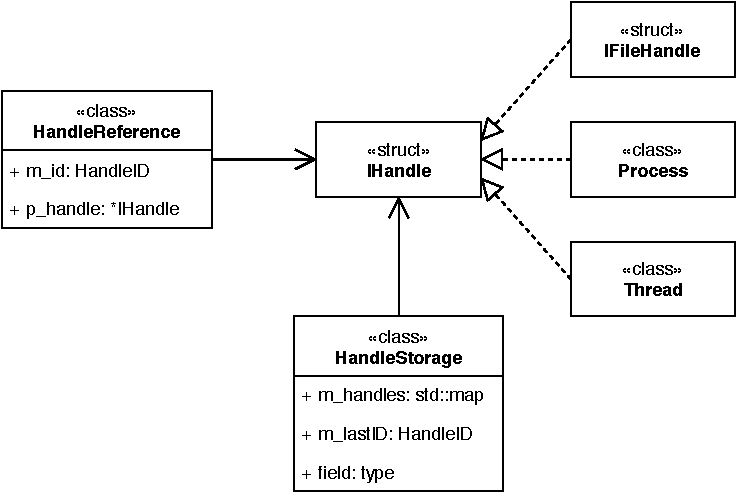
\includegraphics[width=11cm]{handle-class-d.pdf}
		\caption{Diagram tříd handlerů}
		\label{fig:handle-class-d}
	\end{figure}
	
	Uvnitř \verb|HandleStorage| je pro každý handle uložen počet referencí na tento handle, který se inkrementuje vždy při vytvoření nové \verb|HandleReference| a dekrementuje při odstranění \verb|HandleReference|. Handly s nulovým počtem referencí jsou automaticky uzavřeny a odstraněny ze systému. 
	
	Každý proces si udržuje vlastní množinu referencí na handly, které byly v jeho kontextu vytvořeny nebo jinak získány (například při vytváření procesu předá rodičovský proces nově vytvořenému procesu handle na \verb|stdin| a \verb|stdout|). Tato množina se zároveň používá i pro zjištění, zda má proces k nějakému handlu vůbec přístup. Při odstranění nějakého procesu potom dojde k odstranění všech handle referencí uložených v jeho množině, a tím dojde automaticky i k odstranění všech handlů, které používal pouze daný proces. 
	
	Kernel se tak nespoléhá na "slušnost" user-space kódu, který by měl vždy použít \verb|CloseHandle|, ale dokáže při ukončení procesu automaticky uklidit všechny nepotřebné handly stejně jako reálný OS. Zároveň tento koncept umožňuje i efektivnější spolupráci více vláken najednou. Při práci s nějakým handle totiž není potřeba zamykat globální zámky, protože pokud pro tento handle existuje alespoň jeden objekt \verb|HandleReference|, tak je zaručeno, že žádné jiné vlákno nemůže tento handle nečekaně odstranit a způsobit tak pád celého systému.
	
	\subsection{Procesy a vlákna}
	
	Procesy jsou uloženy v již zmíněném \verb|HandleStorage| a \verb|HandleID| je bráno jako PID. Stejně tak jsou uložena i vlákna a \verb|HandleID| představuje TID.
	
	Každé vlákno simulovaného OS využívá reálné vlákno fyzického OS (\verb|std::thread|). Kernel dále neobsahuje žádný platform-specific kód, kromě načítání "user.dll". Za hlavní vlákno procesu se považuje jeho první vlákno. Při vytvoření procesu je vždy vytvořeno i jeho hlavní vlákno.
	
	\subsubsection{API}
	K API je přistupováno skrze systémová volání.
	
	\paragraph{Create Process}
	Vytvoří nový proces.
	
	\begin{figure}[H]
		\centering
		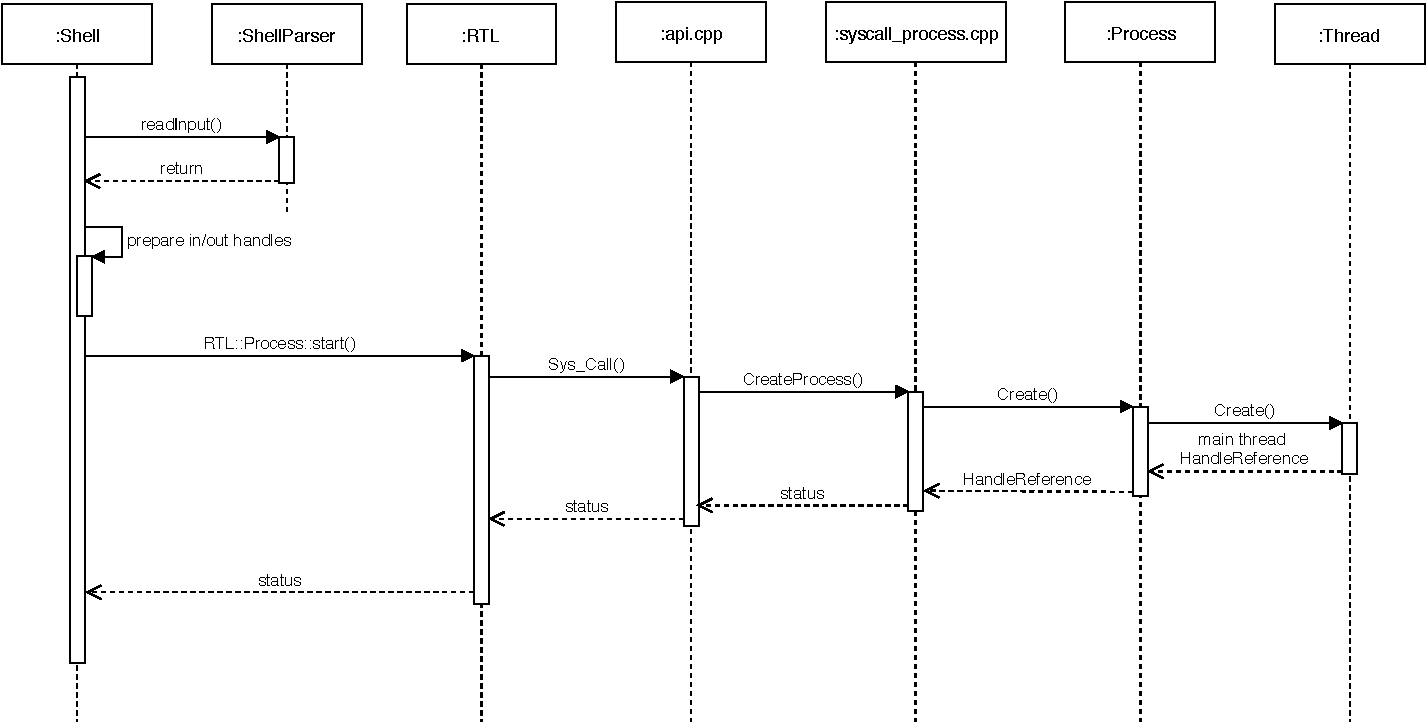
\includegraphics[width=14cm]{create-process-seq.pdf}
		\caption{Sekvenční diagram vytvoření procesu}
		\label{fig:create-process-seq}
	\end{figure}
	
	\paragraph{Create Thread}
	Vytvoří nové vlákno pro aktuální proces.
	
	\paragraph{Wait For}
	Počká na konec procesu, nebo vlákna.
	
	\begin{figure}[H]
		\centering
		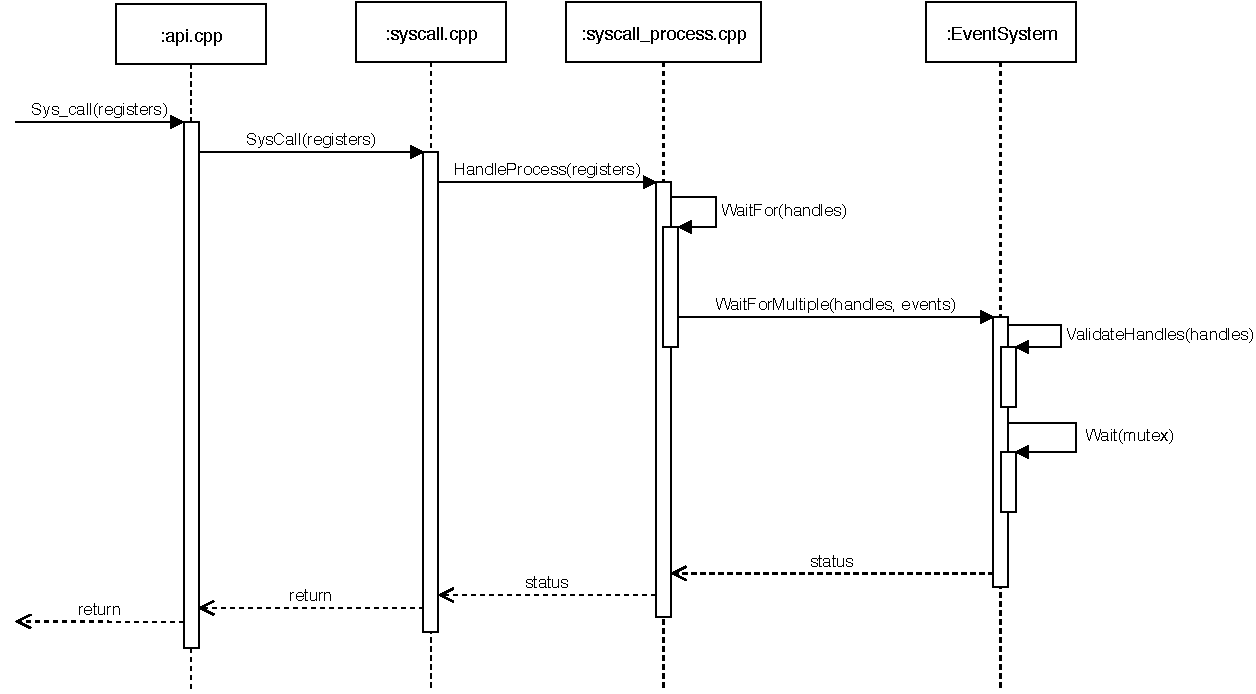
\includegraphics[width=14cm]{wait-for-proc.pdf}
		\caption{Sekvenční diagram čekání na vlákno, nebo proces}
		\label{fig:wait-for-proc}
	\end{figure}
	
	\paragraph{Get Exit Code}
	Získá exit kód procesu, nebo vlákna.
	
	\paragraph{Setup Signal}
	Nastaví signal handler.
	
	\paragraph{Exit}
	Nastaví exit kód aktuálímu vláknu.
	
	\paragraph{System Shutdown}
	Pošle signál terminate na všechna vlákna v systému.

	
	\subsection{Filesystem}
	
	Kernel obsahuje file system manager, který spravuje disky a souborové systémy na nich uložené. Pro přístup na disk je použito abstraktní API, které implementuje každý ovladač pro FS. Struktura je znázorněna na obrázku \ref{fig:fs-layers}. 
	
	\begin{figure}[H]
		\centering
		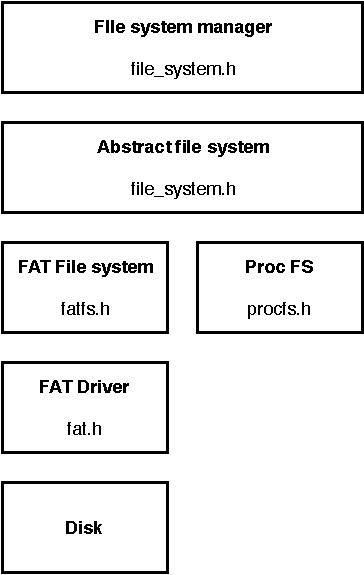
\includegraphics[height=9cm]{fs-layers.pdf}
		\caption{Struktura správy souborového systému}
		\label{fig:fs-layers}
	\end{figure}

	\paragraph{Otevřené soubory} Handly uložených souborů jsou uložené ve výše zmíněném \verb|HandleStorage| -- třída \verb|File|, která představuje handle otevřeného souboru, dědí od \verb|IFileHandle|. K synchronizaci přístupu více vlákny je použit mutex (\verb|std::mutex|). 
	
	\subsubsection{API}
	K datům každého souborového systému je přistupováno skrze API definované v \verb|IFileSystem|. Uživatelská vrstva pak k API přistupuje skrze systémová volání.
	
	\paragraph{Create}
	Vytvoří soubor.
	
	\paragraph{Query}
	Získá info o souboru.
	
	\paragraph{Read}
	Přečte soubor (nebo jeho část) do bufferu.
	
	\paragraph{ReadDir}
	Načte soubory v adresáři.
	
	\paragraph{Remove}
	Odstraní soubor, nebo adresář.
	
	\paragraph{Resize}
	Změní velikost souboru.
	
	\paragraph{Write}
	Zapíše data do souboru.
	
	\subsubsection{FAT}
	
	Jako filesystem jsme zvolili FAT implementovanou v rámci KIV/ZOS. Rozložení souborového systému na disku je znázorněno na obrázku \ref{fig:fat-disk-struct}. V původní specifikaci je na disku uložena alespoň jedna další kopie FAT tabulky, která se používá ke kontrole bloků dat. Protože kontrolu poškozených dat v práci neprovádíme, rozhodli jsme se ukládat pouze jednu kopii.
	
	\begin{figure}[H]
		\centering
		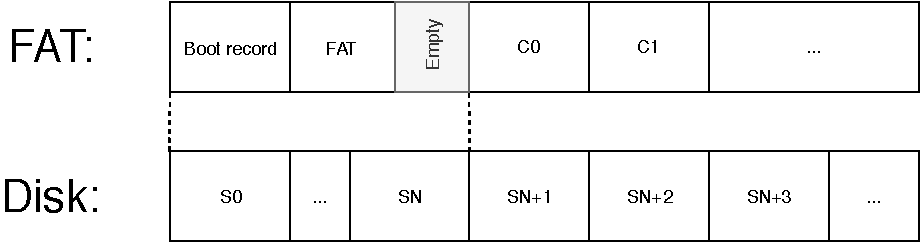
\includegraphics[width=12cm]{fat-rozdeleni-disku.pdf}
		\caption{Uložení FAT souborového systému na disk}
		\label{fig:fat-disk-struct}
	\end{figure}

	Velikost jednoho datového clusteru je dána velikostí sektorů na disku a platí, že 1 cluster = N $\times$ sektor, kde $N$ je vypočítané při inicializaci souborového systému na disku. Root adresář začíná na clusteru 0. Metadata každého souboru jsou reprezentována strukturou \verb|Directory| (obrázek \ref{fig:dir-c}). Adresáře jsou od souborů odlišeny nastaveným bitem ve \verb|flags|.
	
	\begin{figure}[H]
		\centering
		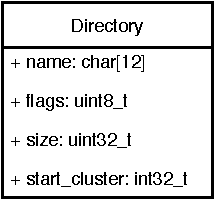
\includegraphics[width=3cm]{dir-c.pdf}
		\caption{Struktura Directory}
		\label{fig:dir-c}
	\end{figure}


	\subsubsection{ProcFS}
	\label{sec:proc-fs}
	Přístup k aktuálně běžícím procesům je realizován přes virtuální souborový systém, který je mapován na disk \verb|0:\|. Struktura je znázorněna na \ref{fig:procfs-struct}. V kořenovém adresáři existuje pro každý běžící proces adresář pojmenovaný podle \verb|HandleID| daného procesu. Adresář pak obsahuje popisné soubory, ze kterých je možné o procesu přečíst: parametry se kterými byl spuštěn, aktuální pracovní adresář, jméno a počet běžících vláken.
	
	\begin{figure}[H]
		\centering
		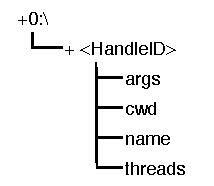
\includegraphics[width=3cm]{procfs-struct.pdf}
		\caption{Struktura ProcFS}
		\label{fig:procfs-struct}
	\end{figure}
	
	\verb|ProcFS| dědí od \verb|IFileSystem| a implementuje tedy celé API pro přístup k datům. Všechny funkce kromě \verb|query()|, \verb|read()| a \verb|readDir()| vrací chybu \verb|PERMISSION_DENIED|. K vypsání všech běžících procesů lze použít funkce \verb|readDir(0:\)|.
	
	Detaily libovolného procesu je možné získat voláním \verb|read(0:\<HandleID>\<proc_file_name>)|. Místo \verb|HandleID| lze použít \verb|self|, API pak vrací detaily o aktuálně běžícím procesu.

	
	\subsection{Roura}
	
	Roura je tvořena dvěma propojenými handly - \verb|PipeReadEnd| a \verb|PipeWriteEnd| viz obrázek \ref{fig:pipe-c}. Čtecí konec obsahuje buffer, do kterého se zapisuje ze zapisovacího konce (metoda \verb|push()|). Při uzavření jednoho konce se spojení mezi nimi přeruší a druhý konec tak ví, že už při prázdném bufferu nemá čekat na další data (čtecí konec) nebo při plném bufferu čekat na uvolnění místa (zapisovací konec).
	
	\begin{figure}[H]
		\centering
		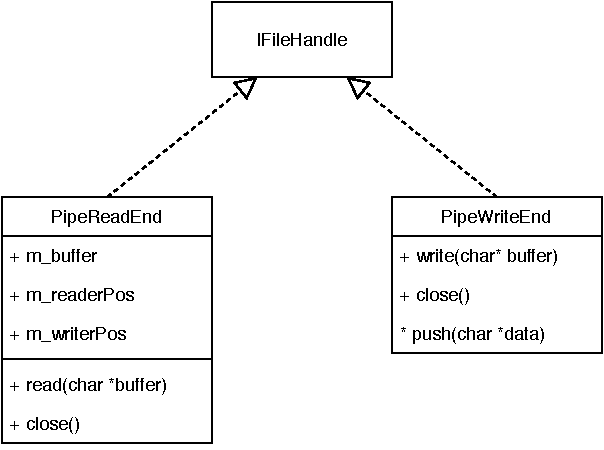
\includegraphics[width=8cm]{pipe-c.pdf}
		\caption{Pipe diagram tříd}
		\label{fig:pipe-c}
	\end{figure}
	
	\section{RTL}
	Vrstva mezi uživatelskými programy a kernelem (nečekaně).
	
	TODO: něco napsat sem? Asi o práci se vstupem/výstupem
	
	\section{Shell a uživatelské příkazy}
	
	\subsection{Parser}
	TODO: informace o parseru
	
	\subsection{Implementace příkazů}
	TODO: nějaký krátký info k příkazům, jak se předává vstup/výstup příkazům
	
	\paragraph{dir}
	Vypíše na výstup seznam souborů v zadaném adresáři. Cest lze příkazu skrze parametry předat více. Příkaz otevře zadaný adresář funkcí \verb|OpenDirectory(path)| z RTL. Obsah adresáře je získán RTL funkcí \verb|GetDirectoryContent(dirHandle)|.
	
	\paragraph{echo}
	Vypíše text ze vstupu na výstup. Echo lze vypnout příkazem \verb|@echo off| (a zapnout \verb|@echo on|). Proměnná, která drží stav echa je uložena v každé instanci shellu zvlášť. K výpisu na výstup je použita funkce RTL \verb|WriteFile(handle)|.
	
	\paragraph{find}
	Najde zadaný text v souboru. Parametry \verb|/C| \verb|/V|.
	
	\paragraph{freq}
	Čte vstup dokud nepřijde EOF a udělá statistiku, kolikrát byl který byte na vstupu přítomen. Po dokončení statistiky je výsledek vypsán na výstup. 
	
	\paragraph{md}
	Vytvoří zadaný adresář. Adresářů lze skrze parametry předat více. Příkaz vytvoří adresář voláním funkce RTL \verb|CreateDirectory(path)|.
	
	\paragraph{rd}
	Smaže zadaný soubor. Použitím parametru \verb|/S| lze rekurzivně mazat adresářové stromy. Soubor je smazán voláním funkce RTL \verb|DeleteDirectory(path)|.
	
	\paragraph{rgen}
	Generuje náhodná čísla v rozmezí $<0;1)$, která vypisuje na výstup. Čísla jsou generována dokud na vstupu není EOF.
	
	\paragraph{shutdown}
	Vypne systém voláním funkce RTL \verb|Shutdown()|.
	
	\paragraph{sort}
	Čte řádky ze vstupu a řadí je. Po přečtení EOF vypíše seřazené řádky na výstup.
	
	\paragraph{tasklist}
	Zavolá \verb|OpenDirectory("0:")| čímž otevře vituální disk 0 (viz sekce \ref{sec:proc-fs}), načte jeho obsah (\verb|GetDirectoryContent()|) a vypíše jej na výstup.
	
	\paragraph{type}
	Vypíše na výstup obsah zadaných souborů. K otevření souboru je použita funkce RTL \verb|OpenFile(path)|, k získání obsahu pak \verb|ReadFile(handle, buffer)|.
	
	\section{Závěr}
	Simulátor operačního systému se nám podařilo úspěšně implementovat. 
	
	TODO: co bychom mohli příště udělat líp 
	
	TODO: co bylo nejzajímavější
	
\end{document}
